\section{Demo}
\begin{frame}
	\begin{center}
		{\fontsize{20}{20}\selectfont
			\textbf{DEMO}
		}
	\end{center}
\end{frame}

\begin{frame}
	\frametitle{CIMIS stations}
	\centering
	\begin{figure}
		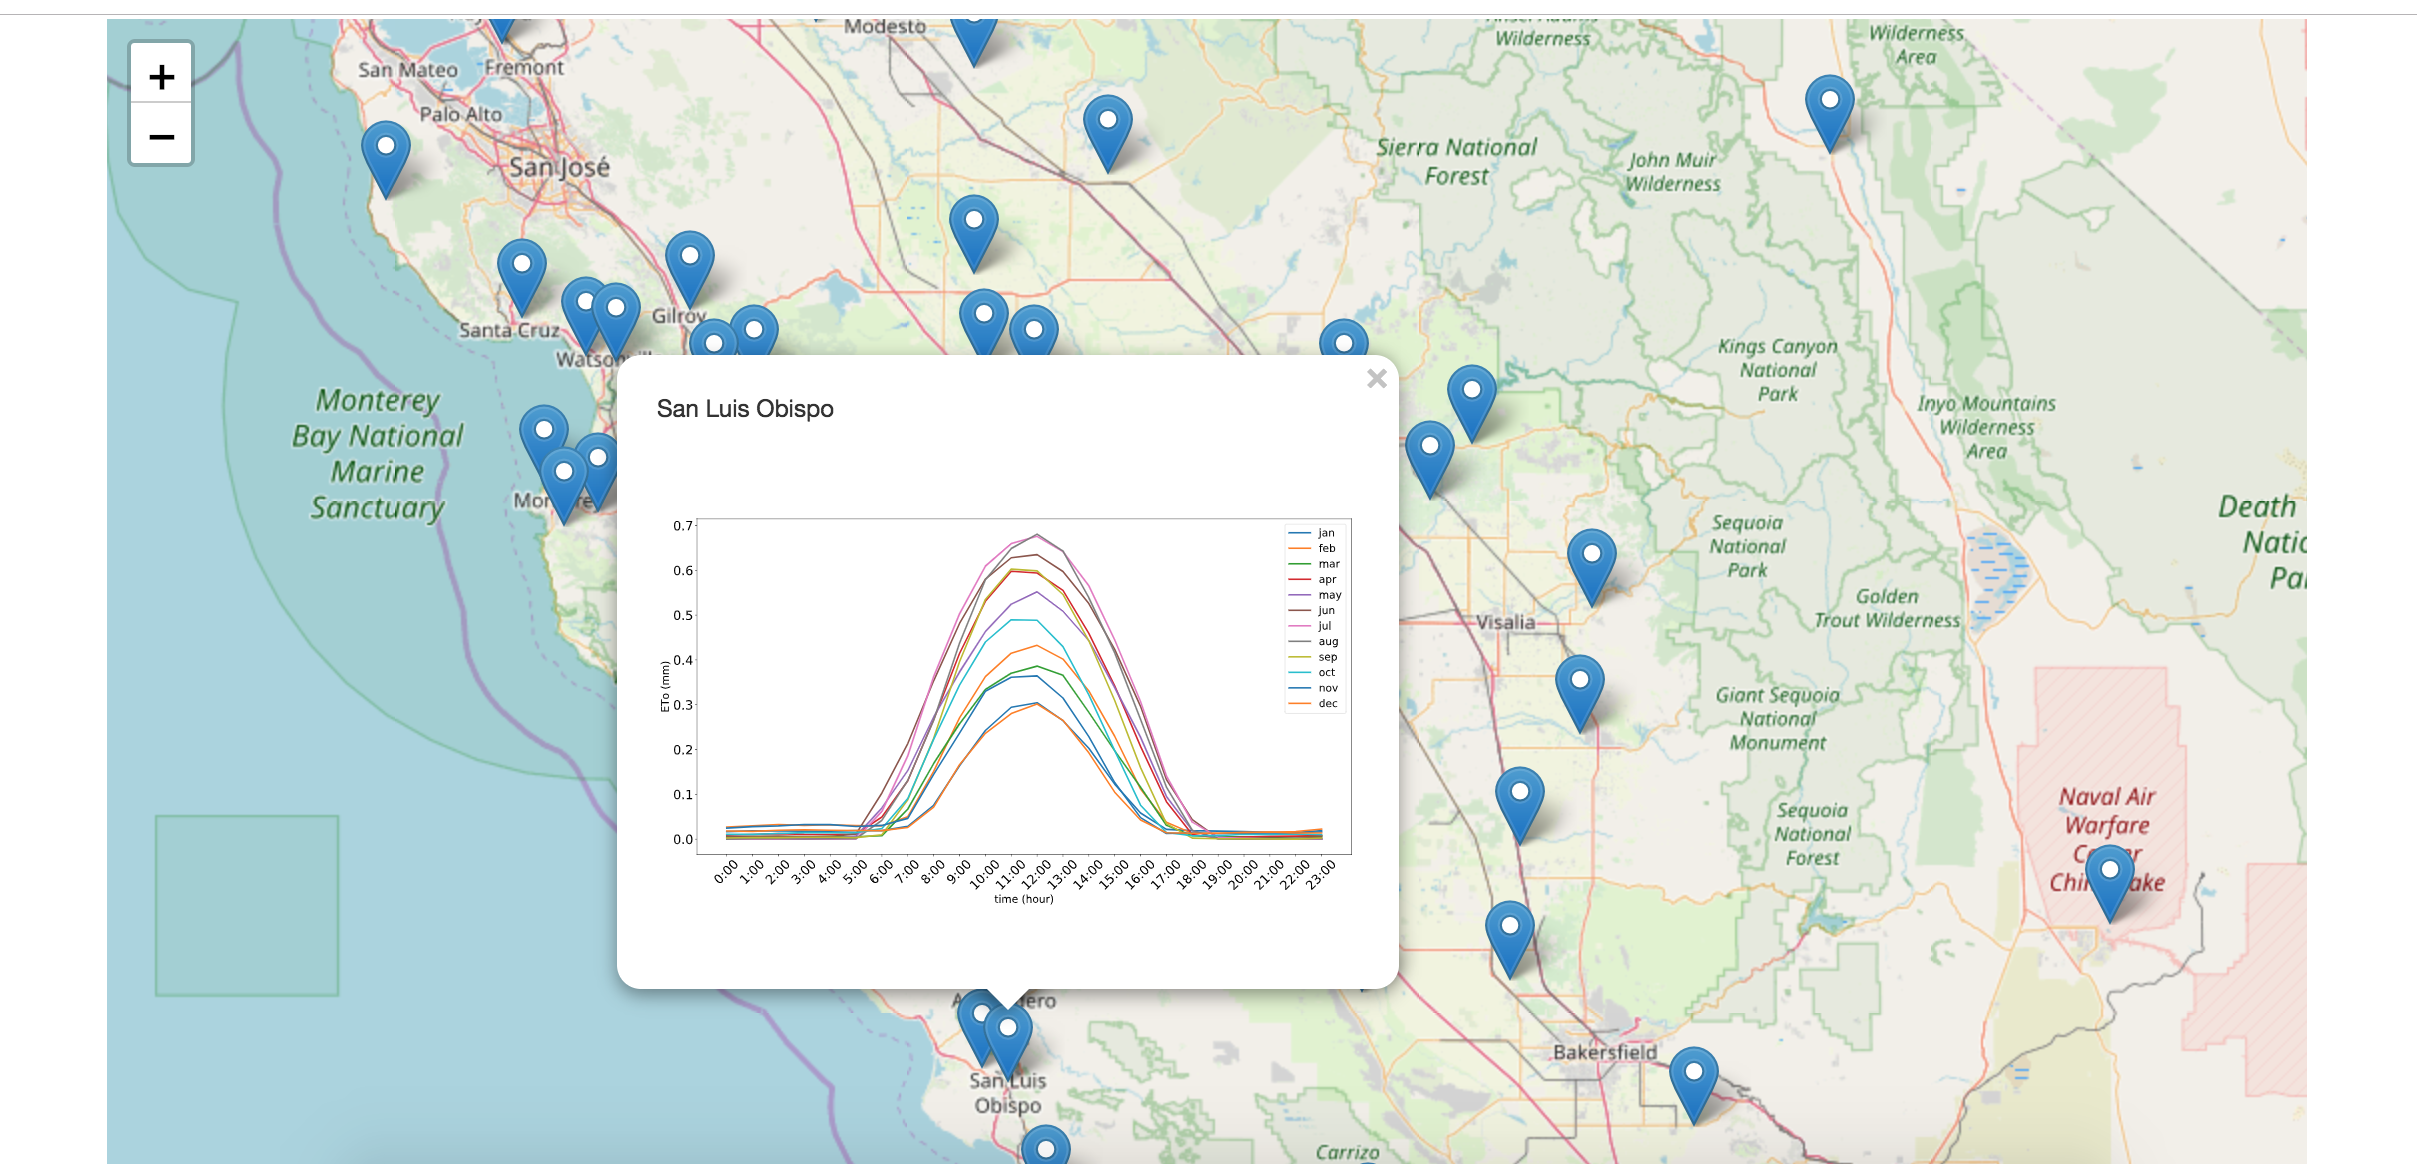
\includegraphics[width=0.9\textwidth]{images/fig1.png}
		\caption{Graph showing the monthly ET values for San Luis Obispo}\label{fig:fig1}
	\end{figure}
\end{frame}

\begin{frame}
	\frametitle{ET values on a particular date}
	\centering
	\begin{figure}
		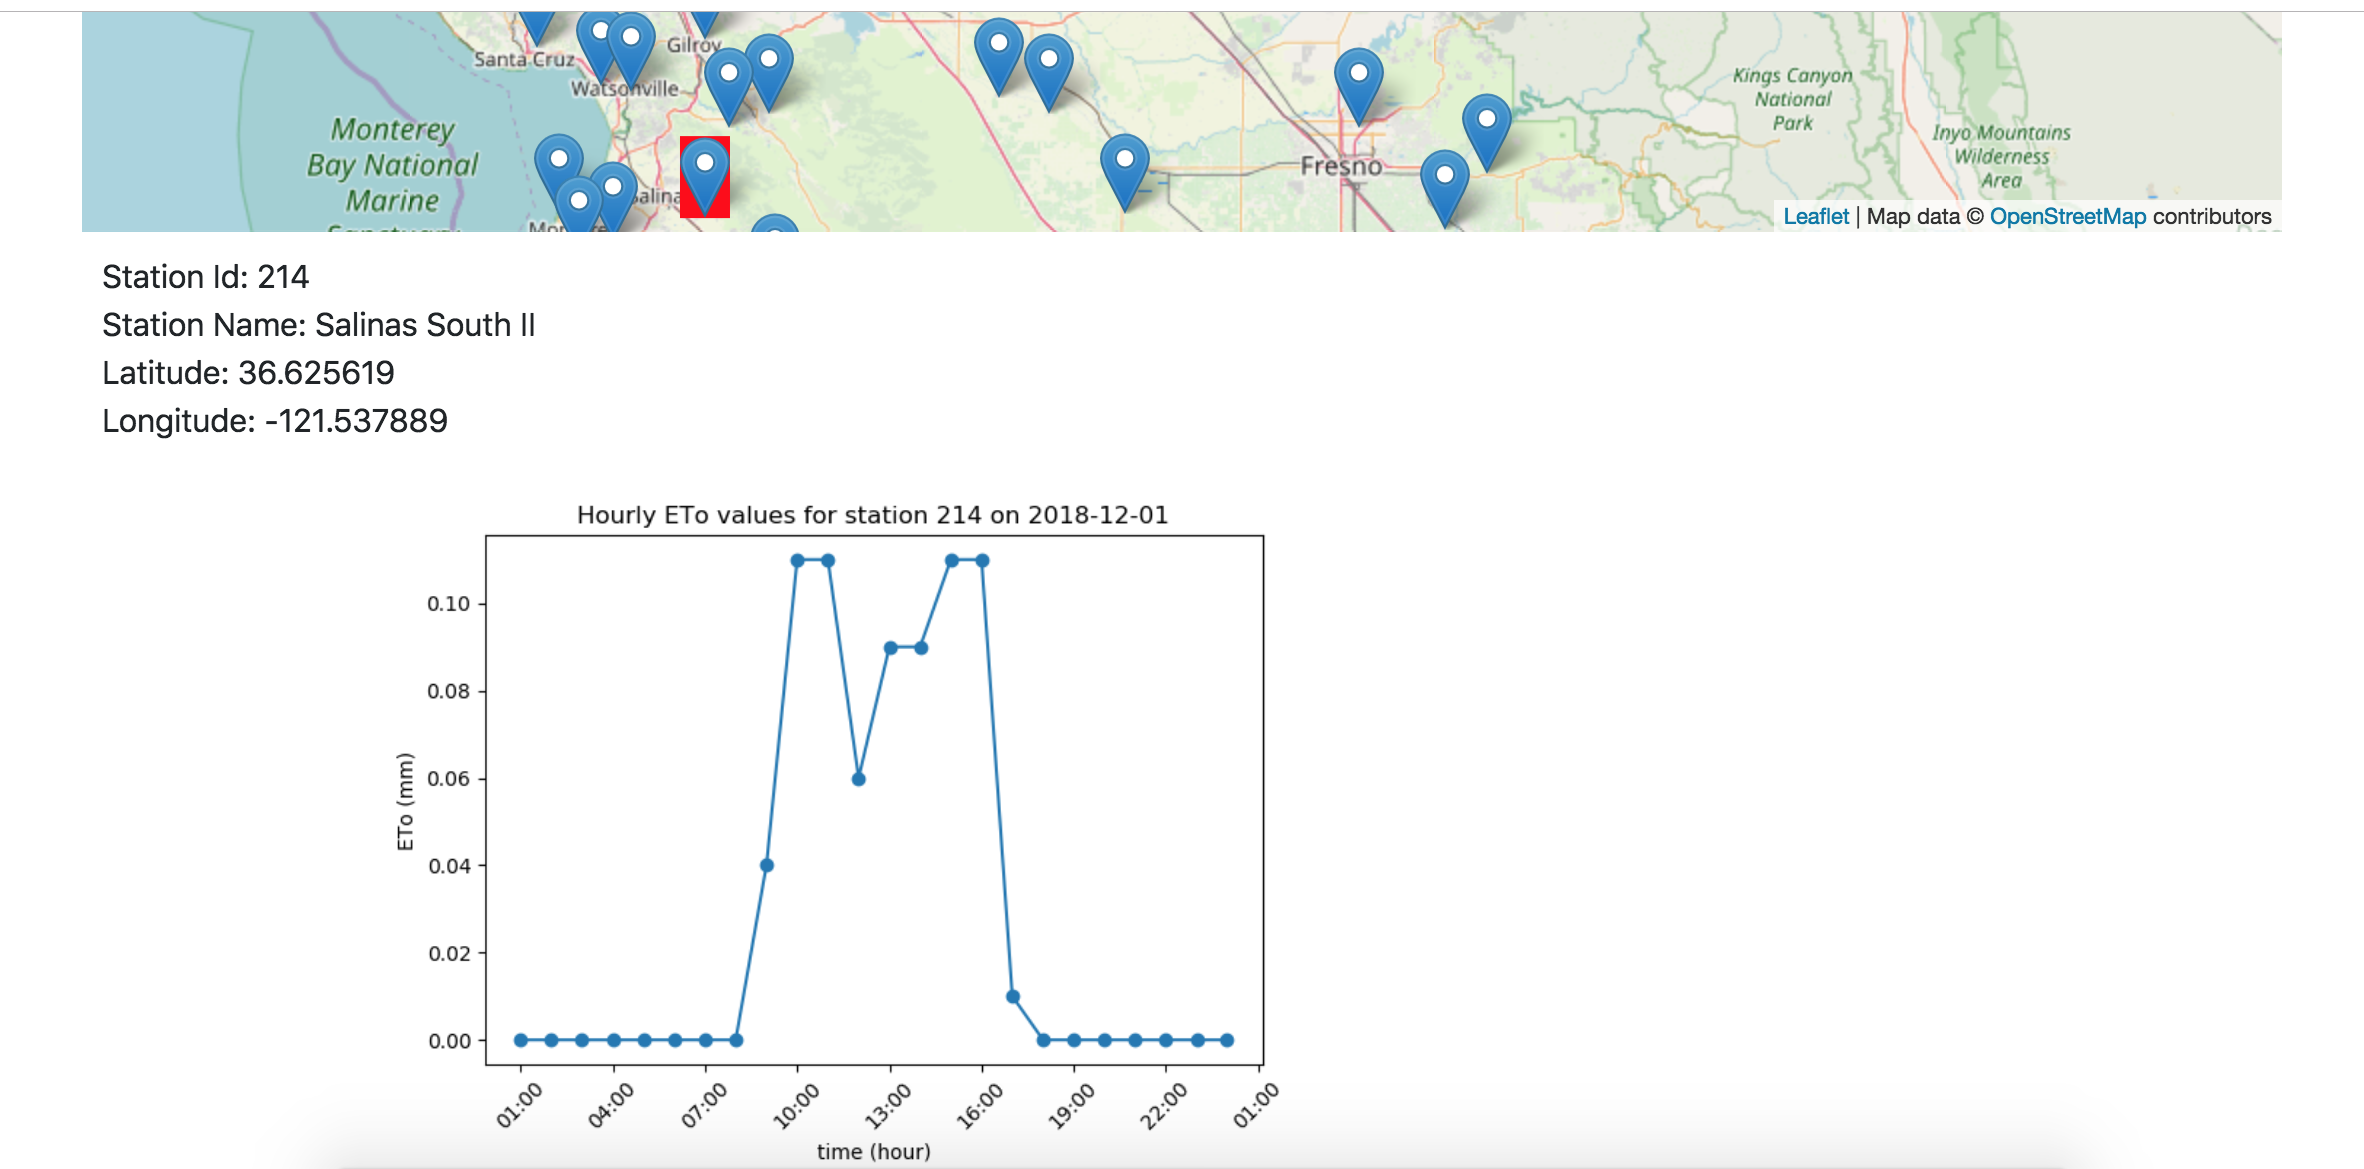
\includegraphics[width=0.9\textwidth]{images/fig2.png}
	\end{figure}
\end{frame}

\begin{frame}
	\frametitle{Linear Regression}
	\centering
	\begin{figure}
		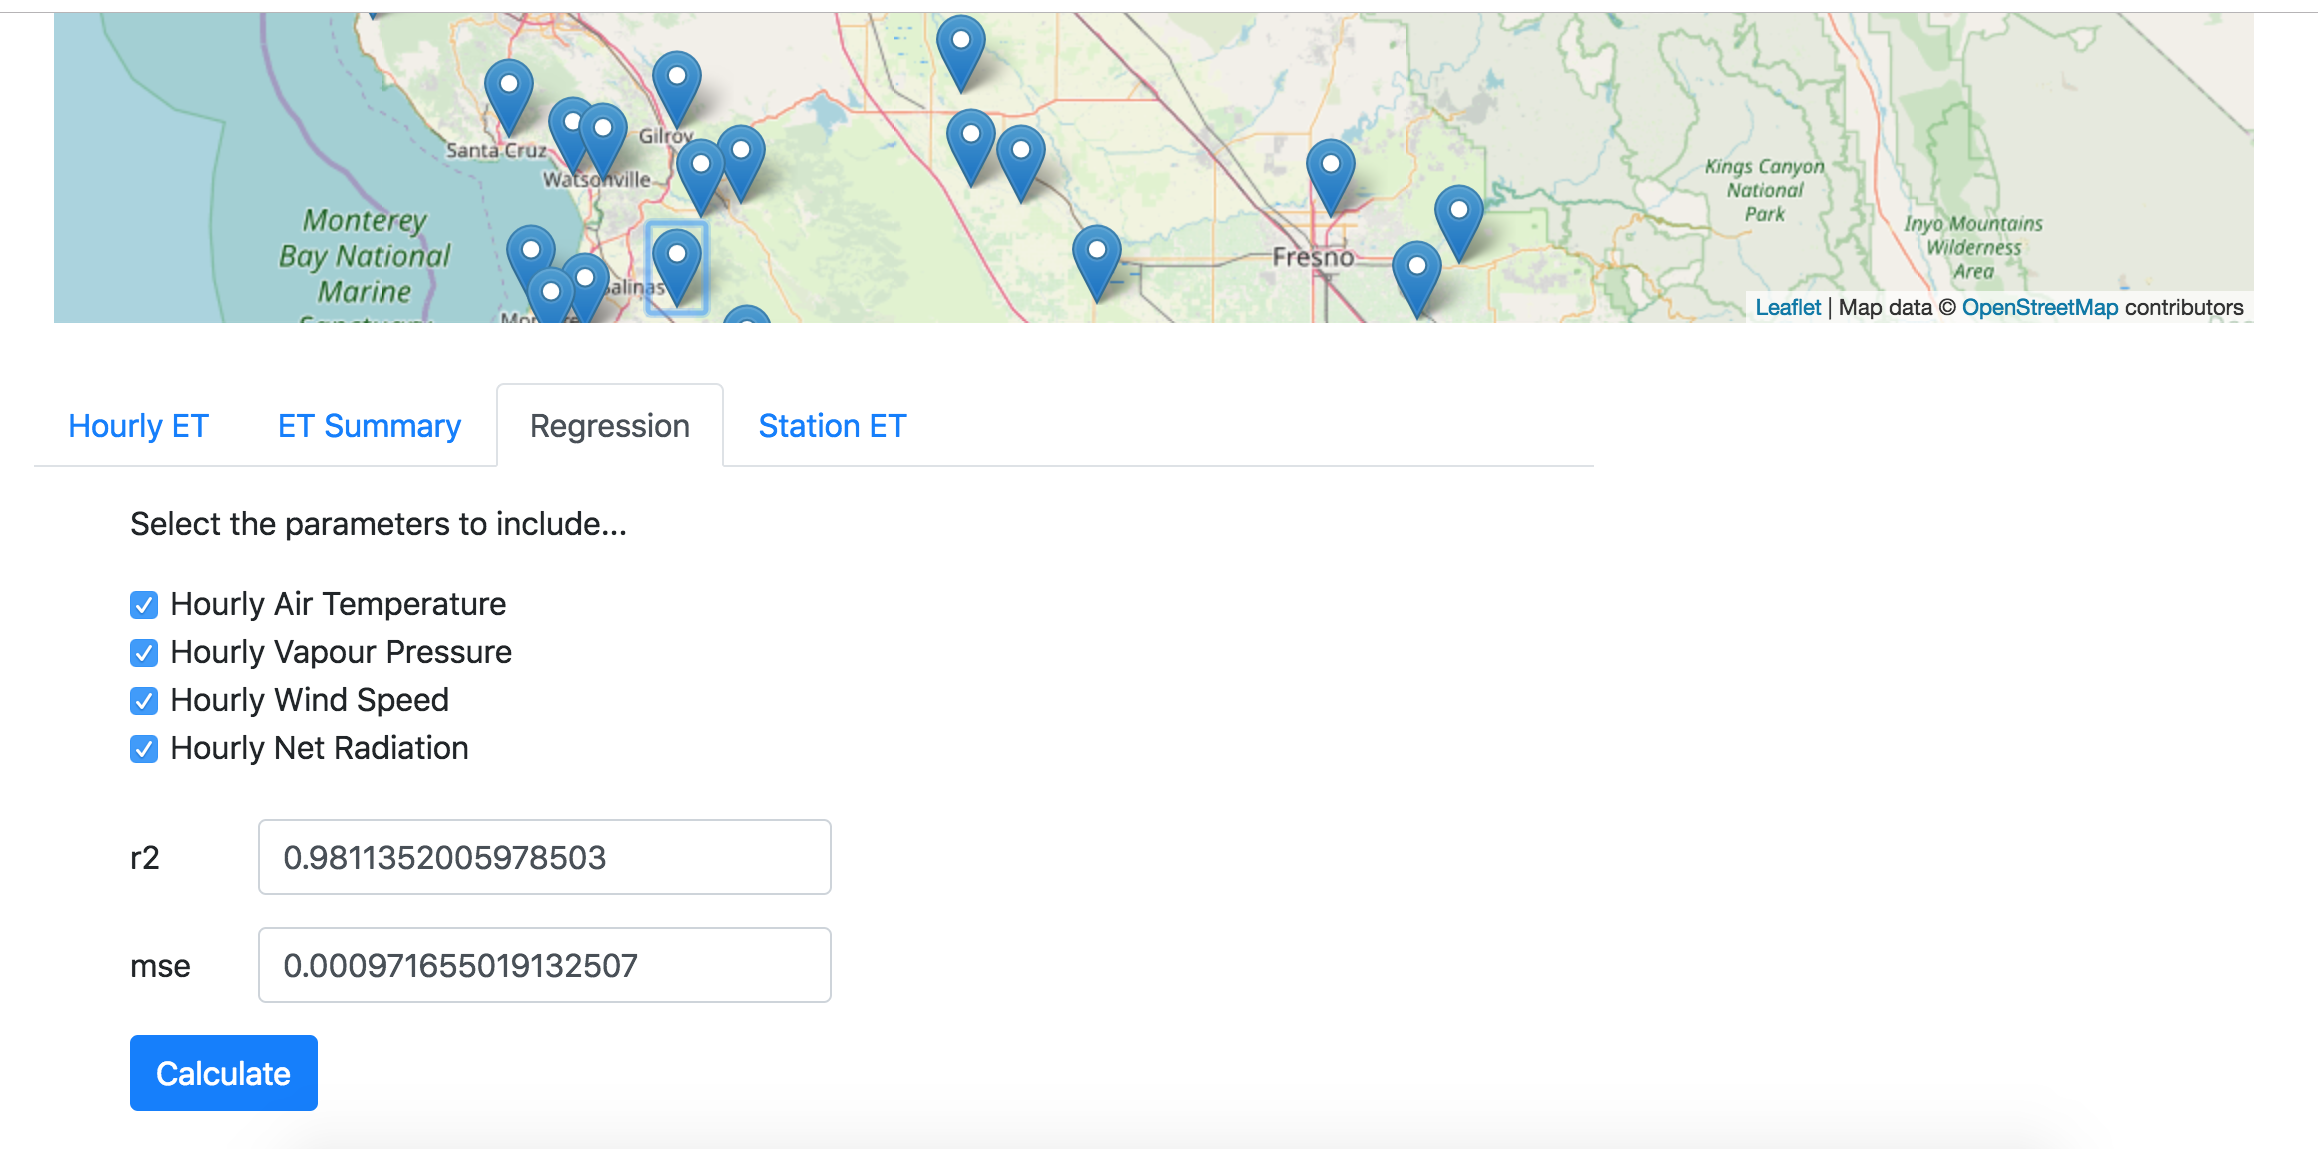
\includegraphics[width=0.9\textwidth]{images/fig3.png}
	\end{figure}
\end{frame}

\begin{frame}
	In Fig.~\ref{fig:2-2016} we can see an example of the typical 12 month graph for one of the stations. There is a even spread between all the months in average
\end{frame}

\begin{frame}
\frametitle{Normal 12-month Graph for Station 2 in 2016}
\centering
\begin{figure}
	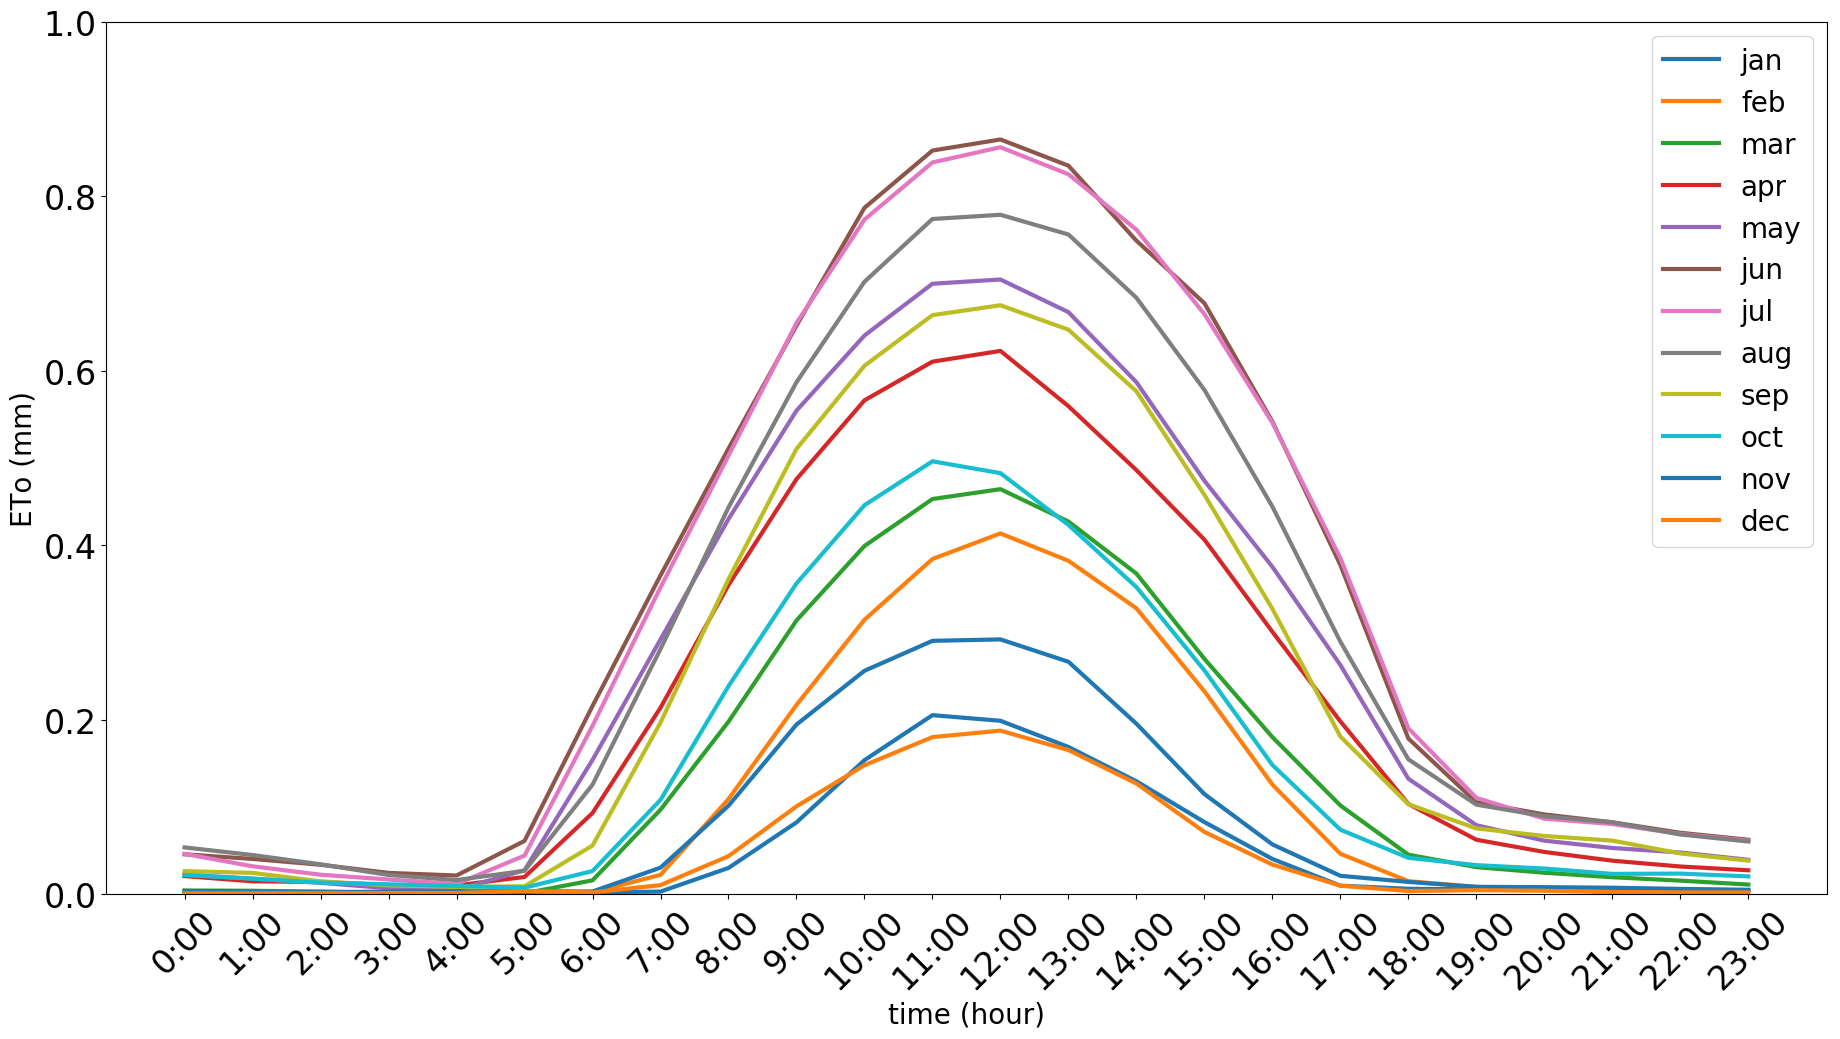
\includegraphics[width=0.9\textwidth]{images/2-2016.png}
	\caption{Normal 12-month Graph for Station 2 in 2016}\label{fig:2-2016}
\end{figure}
\end{frame}

\begin{frame}
	In Fig.~\ref{fig:12-2016} 
\end{frame}

\begin{frame}
\frametitle{12-month Graph for Station 12 in 2016}
\centering
\begin{figure}
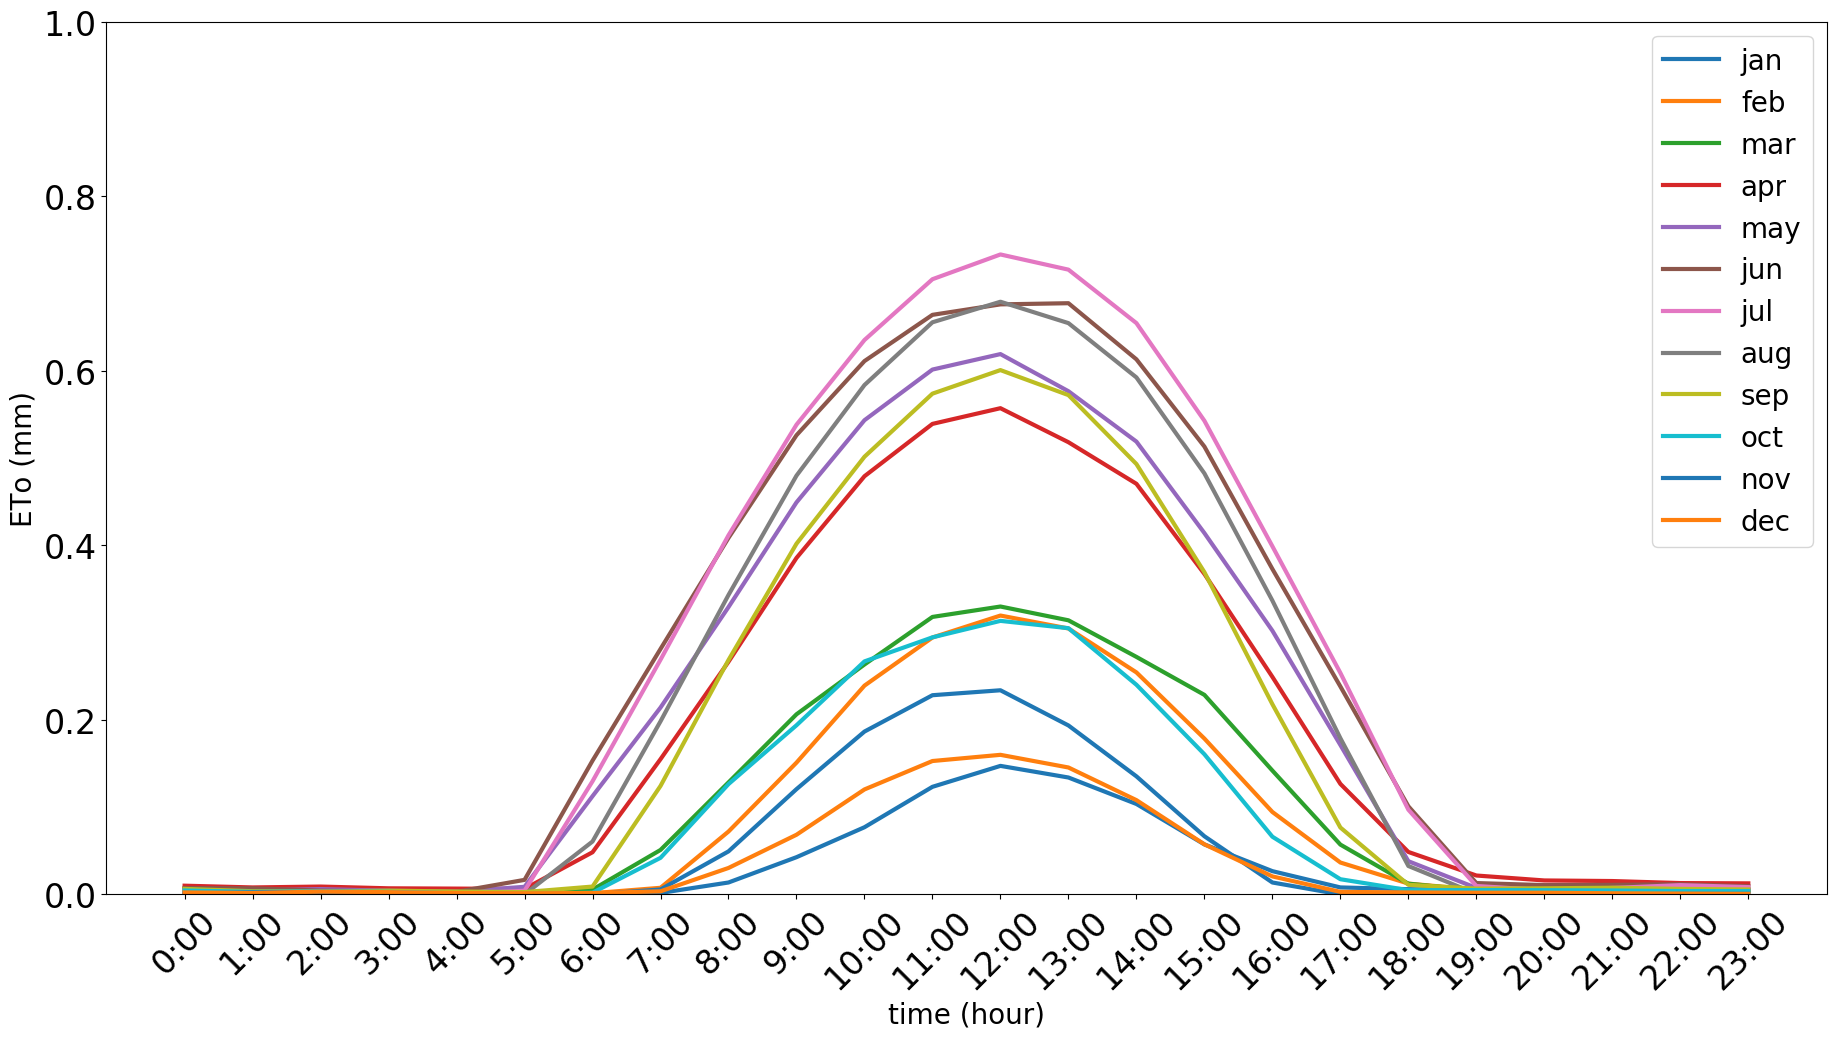
\includegraphics[width=0.9\textwidth]{images/12-2016.png}
\caption{12-month Graph for Station 12 in 2016}\label{fig:12-2016}
\end{figure}
\end{frame}

\begin{frame}
\frametitle{12-month Graph for Station 62 in 2018}
\centering
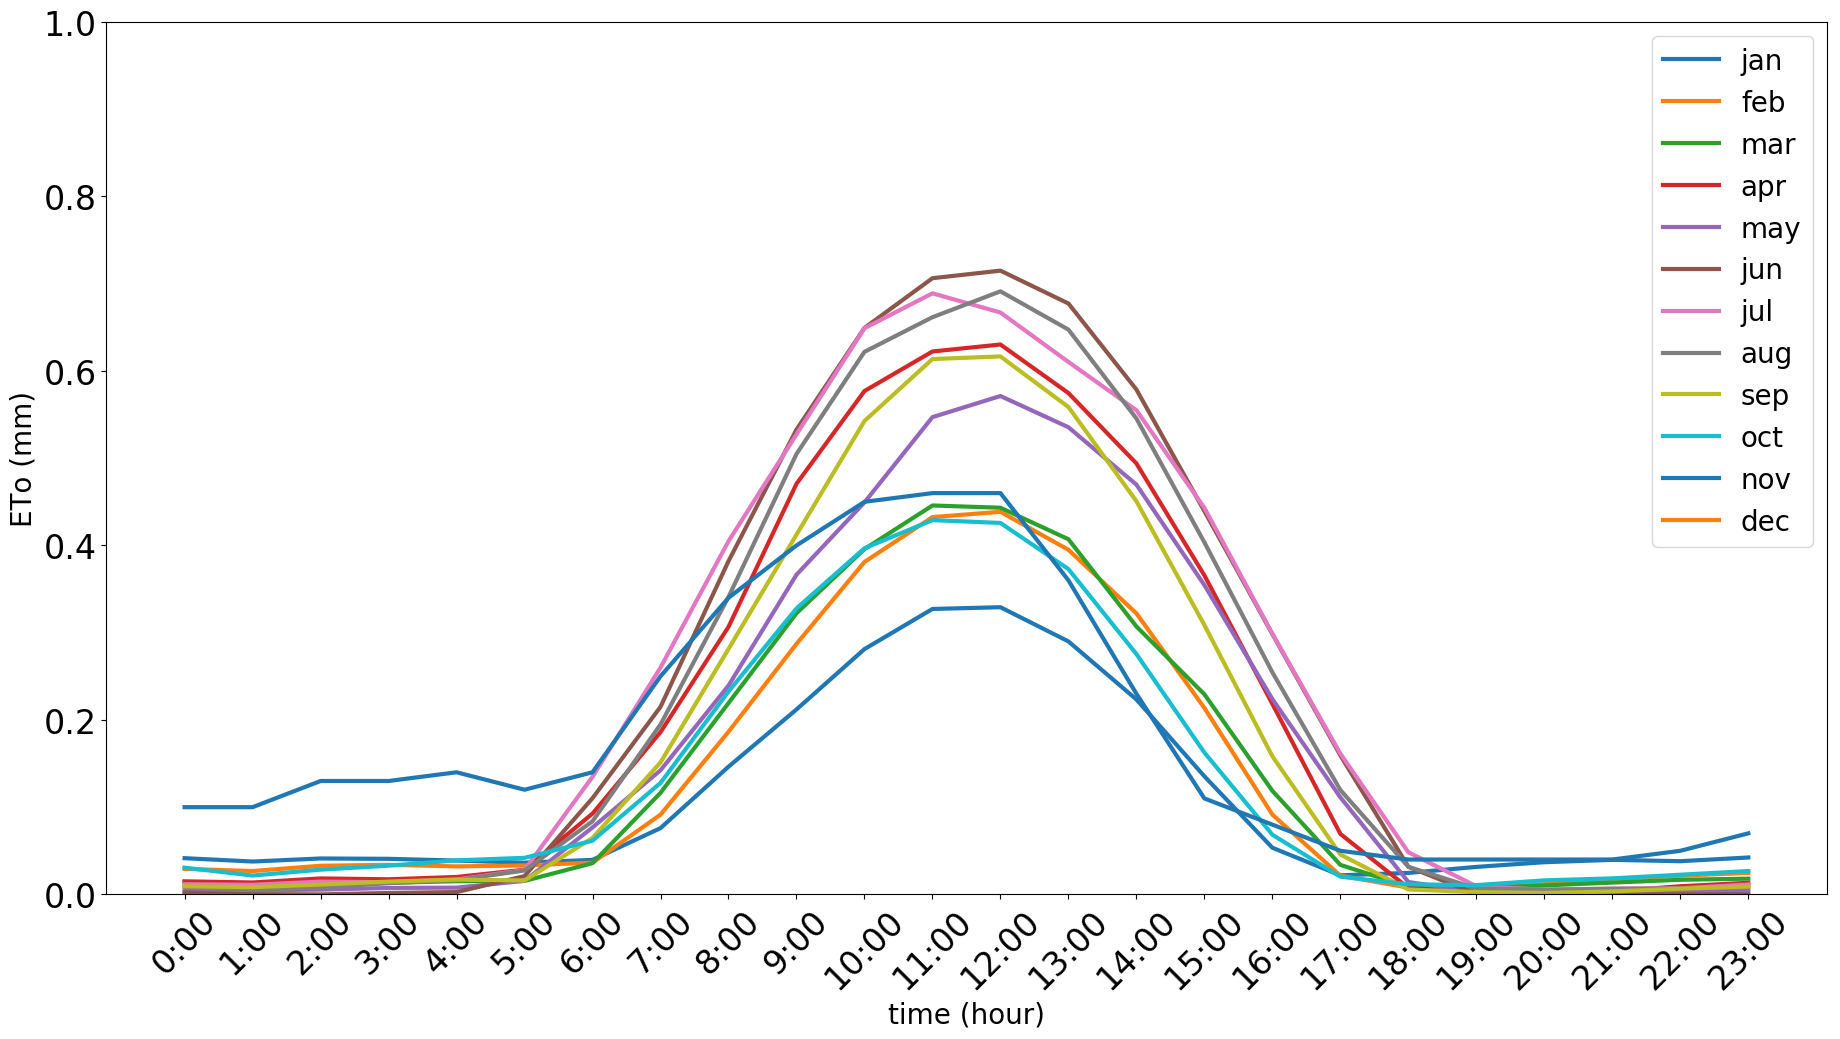
\includegraphics[width=0.9\textwidth]{images/62-2018.png}
\end{frame}

\begin{frame}
\frametitle{36-month Graph for Station 2}
\centering
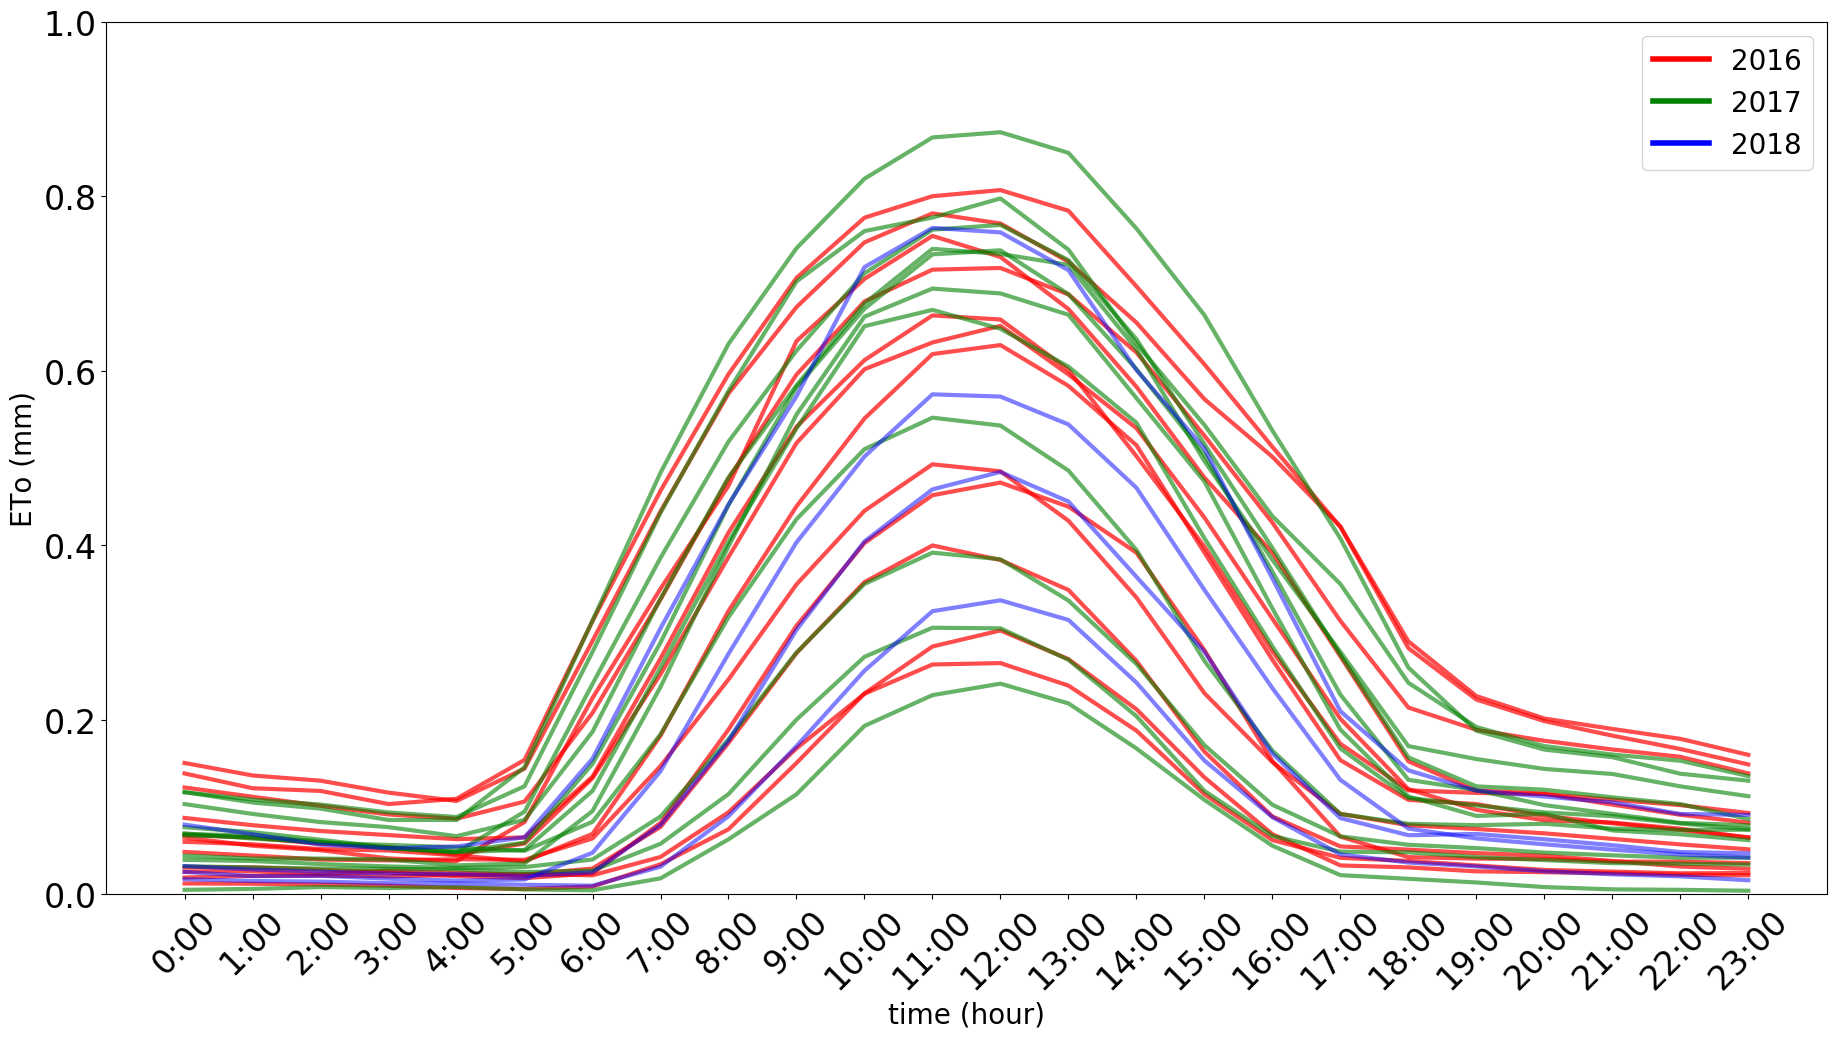
\includegraphics[width=0.9\textwidth]{images/234multi.png}
\end{frame}



\begin{frame}
\frametitle{36-month Graph for Station 7}
\centering
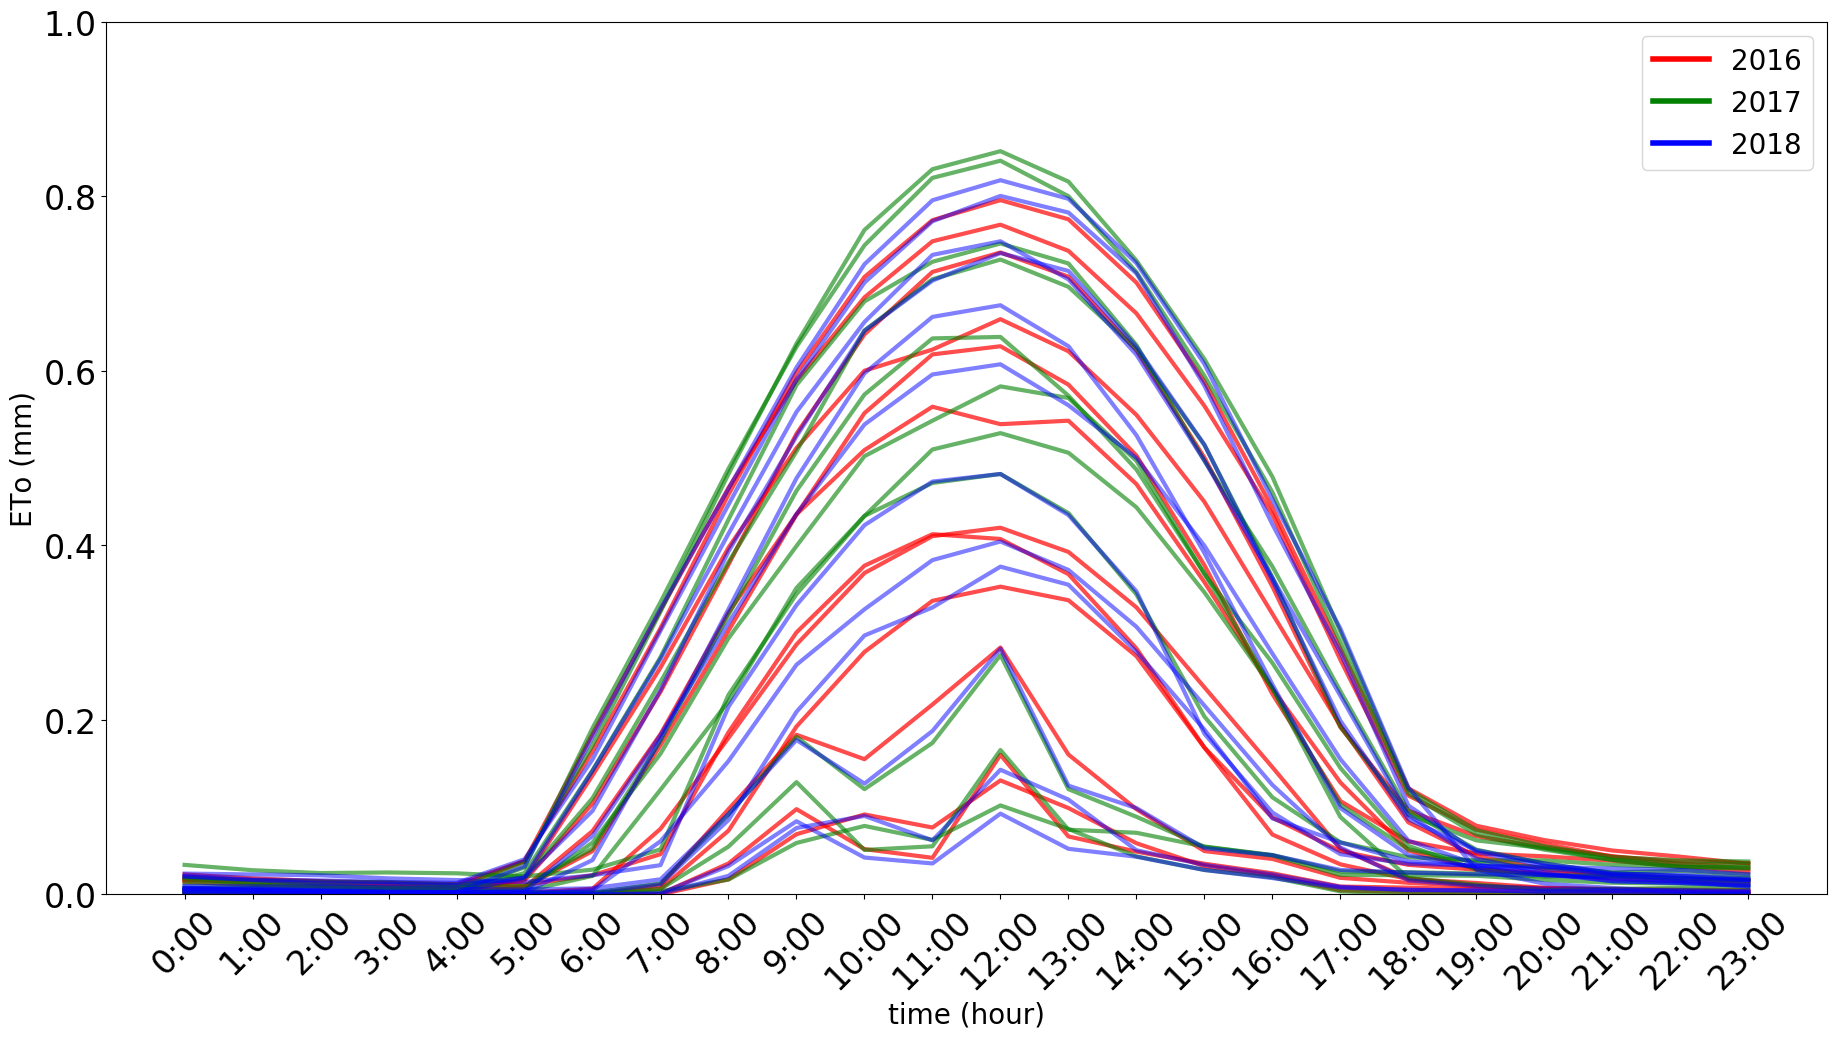
\includegraphics[width=0.9\textwidth]{images/7multi.png}
\end{frame}


\begin{frame}
\frametitle{36-month Solar Graph for Station 7}
\centering
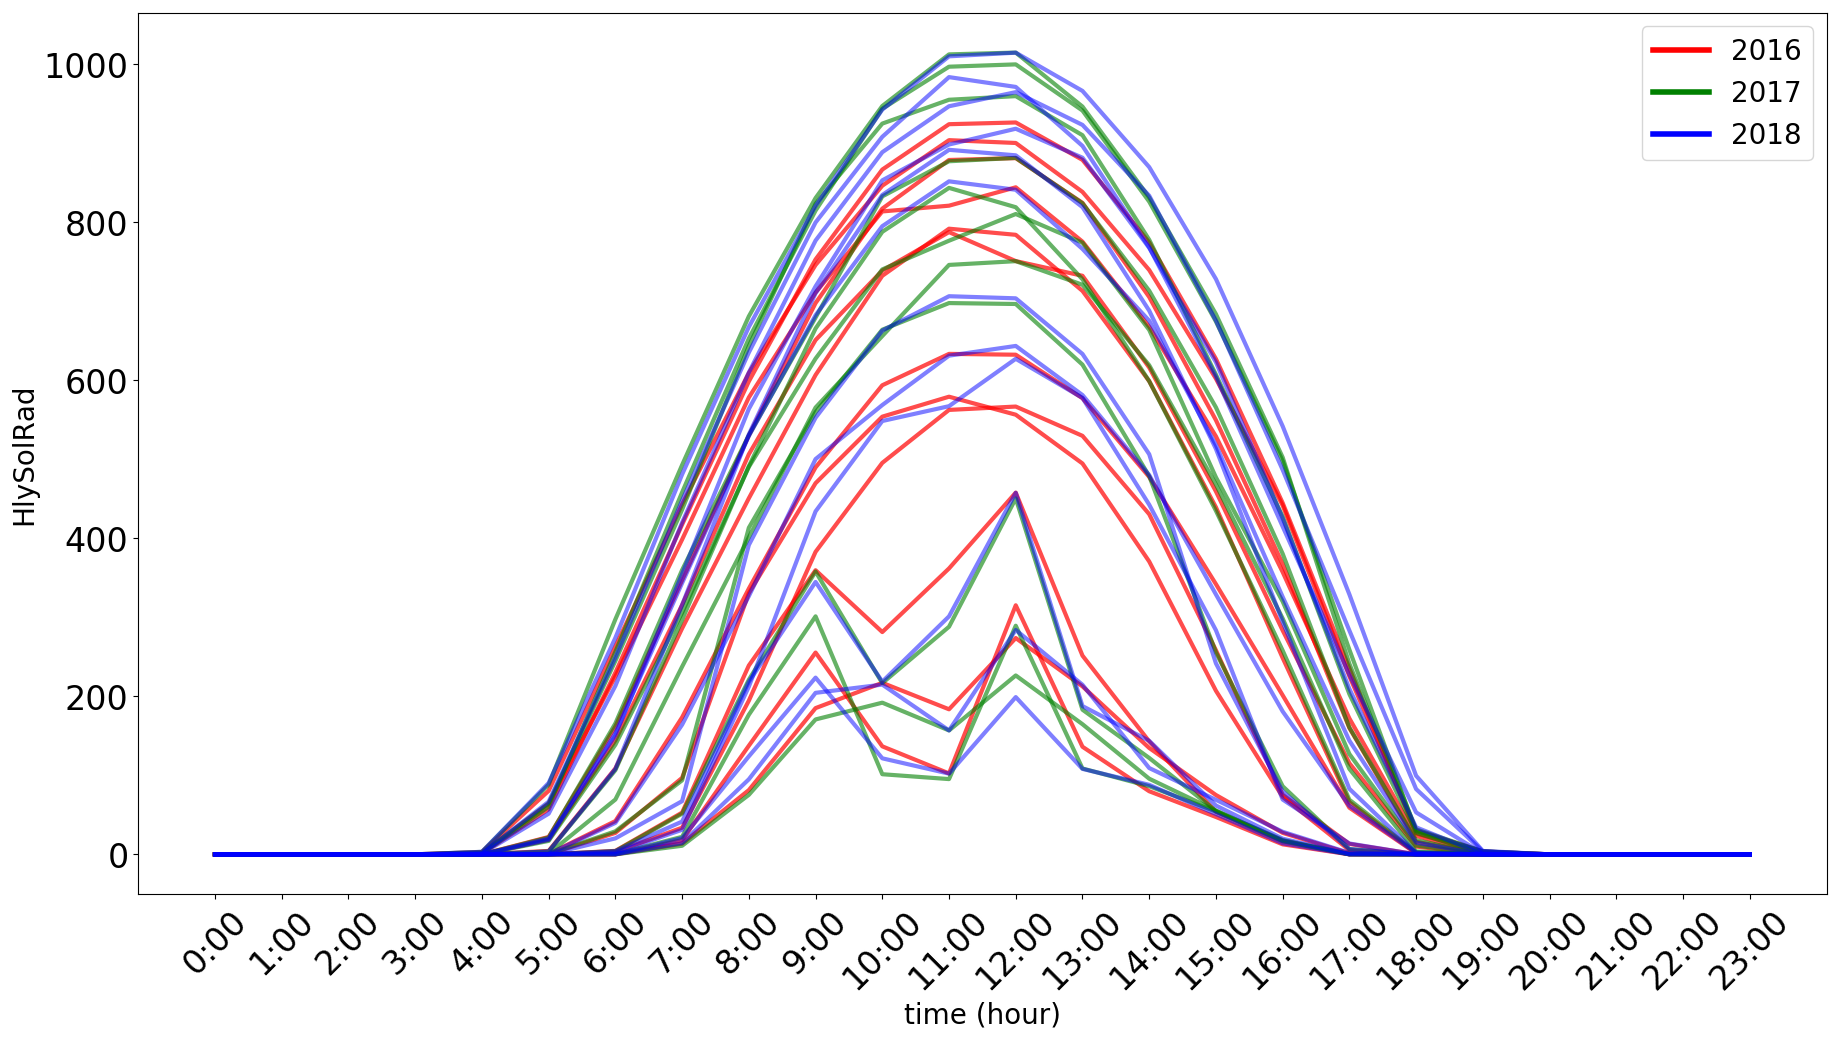
\includegraphics[width=0.9\textwidth]{images/3year7solar.png}
\end{frame}


\begin{frame}
\frametitle{36-month Graph for Station 202}
\centering
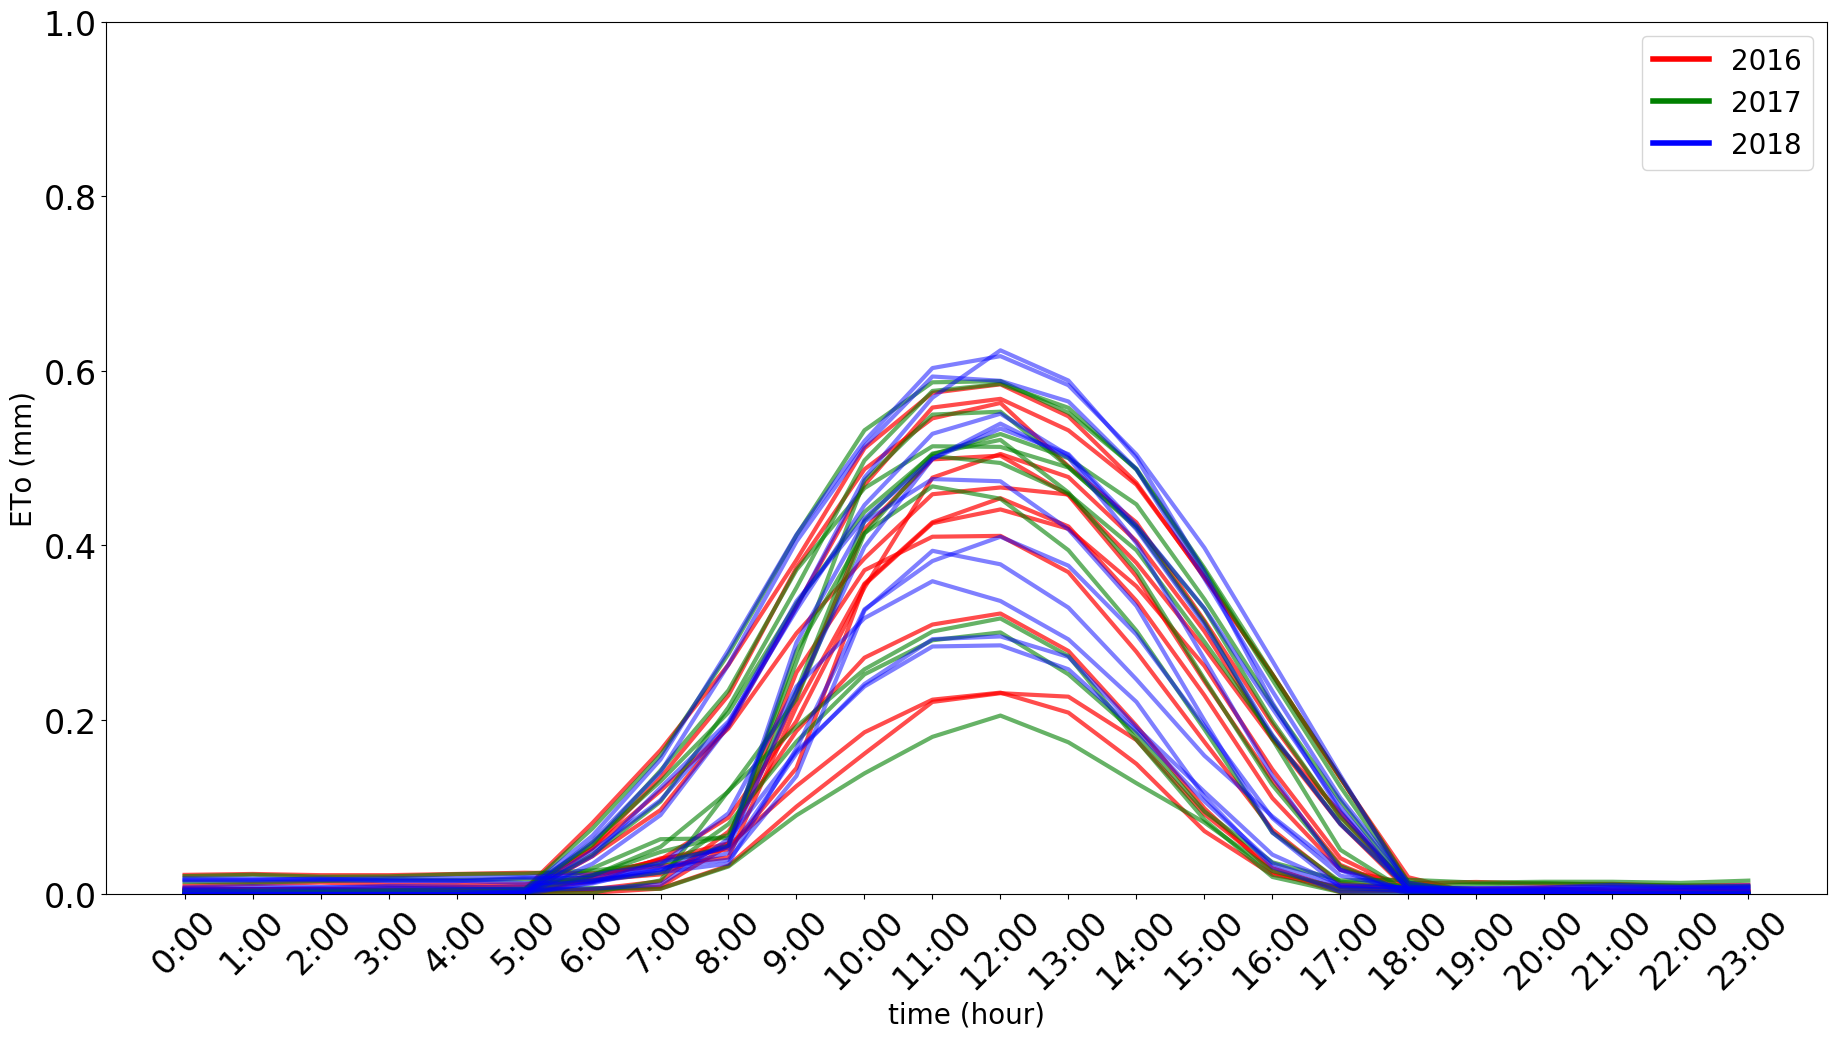
\includegraphics[width=0.9\textwidth]{images/202multi.png}
\end{frame}

